% !TeX encoding = utf8
% !TeX root = ./main.tex


% -------------------------------------------------------------------------
\chapter{引言}
% -------------------------------------------------------------------------

\section{研究背景与意义}

\begin{figure}
	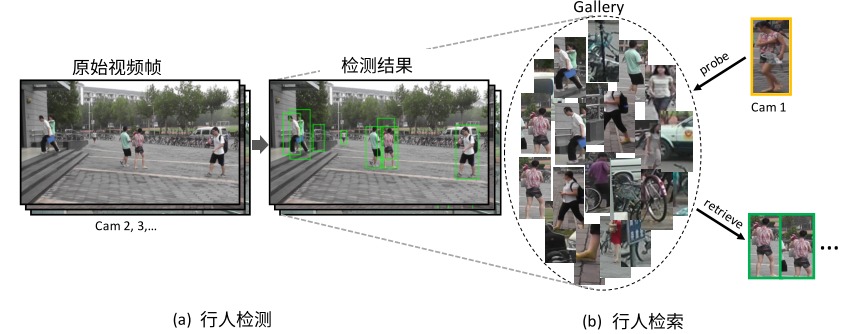
\includegraphics[width=\textwidth]{fig/background.png}
	\caption{广义的行人再识别任务的总体框架,图片修改自~\cite{zheng2017person}}
	\label{fig:overall}
\end{figure}

近年来,随着城市安防越来越被重视,安防监控系统越来越普及。
复杂的摄像头网络和海量的视频数据,使得依赖人力观察每个监控设备视频的方法不再适用。
智能行人监控技术应运而生,其中行人再识别(Person Re-identification, Person Re-ID)作为智能行人监控系统的核心技术之一,成为一个新的研究热点。
近几年,行人再识别领域投稿数量和性能均大幅增长,
2015年性能指标CMC-1(Cumulative Matching Characteristic with Rank-1, 只考虑第一个预测结果的累计匹配因子)
只有$65\%$。17年达到了$80\%-85\%$。随后17年11月,在Arxiv上抢先公布的技术报告已经达到了$90\%-96\%$,号称在大型数据集上超越人类的表现。预计18年行人再识别领域会有更多应用和突破。

图~\ref{fig:overall}为广义的行人再识别过程。
广义的行人再识别可以被分解为三个步骤:行人检测(Pedestrian Detection),
行人跟踪(Pedestrian Tracking),
行人检索(Pedestrian Retrieval)。
其中行人检测是从视频监控视频每一帧中检测出行人的技术;
行人跟踪是在时序上将行人串联起来形成视频片段的技术;
而行人检索是利用得到的行人图像完成跨摄像头行人检索的技术。
根据Zheng \etal \parencite{zheng2017person} 的定义,行人检测和行人跟踪是计算机视觉中已经存在的任务,因此大多研究者所指的狭义的行人再识别问题(Person Re-identification,Person Re-ID)着力解决第三个模块,也即
行人检索问题。
本文也不例外,着力解决狭义的行人再识别问题,也即行人检索问题。

\section{国内外研究现状}

\begin{figure}
	\centering
	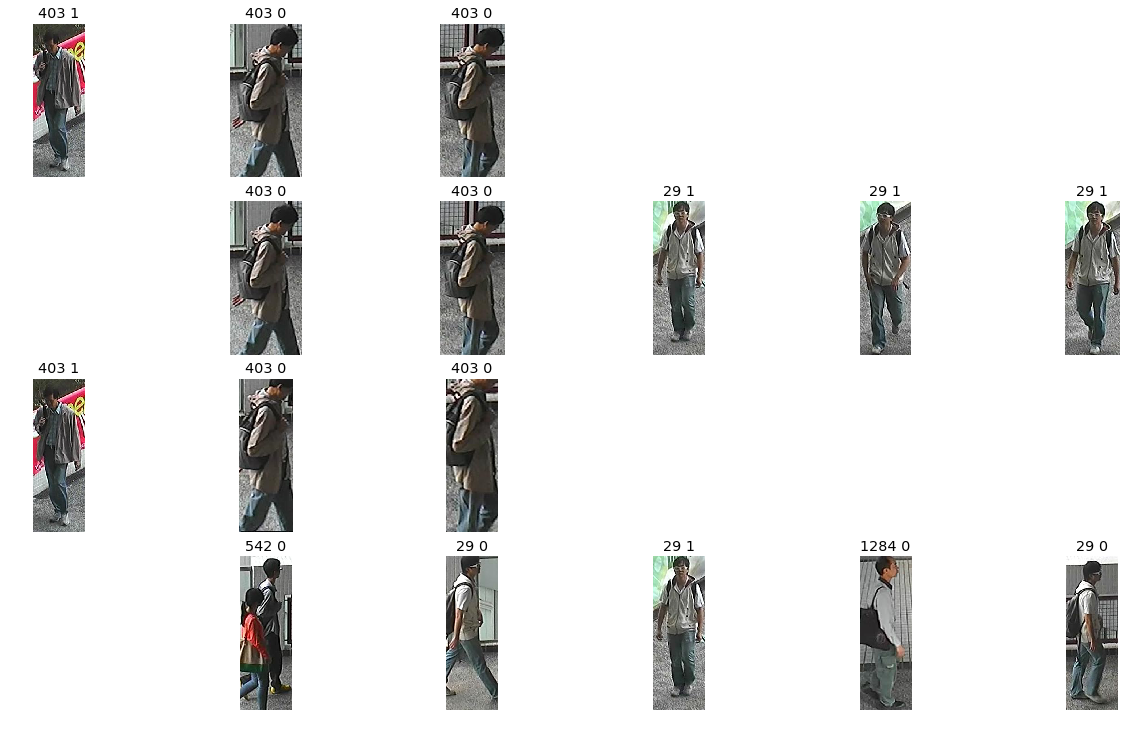
\includegraphics[width=\textwidth]{fig/2018-04-18-21-53-15.png}
	\caption{我们的基准模型在手工标注的数据集和行人检测器自动检测的数据集上的典型样例} \label{fig:label2det}
\end{figure}

行人再识别中存在许多挑战。由于行人的非刚性运动、检测器的误差、摄像头的视角变化,同一行人的不同图片往往存在严重的空间失配(Spatial Misalignment);与人脸图片相比,行人图片没有可靠的生物特征,只能从属性、语义层面的特征加以区分;未标定的摄像机参数、巨大的时空跨度,这些都进一步增加了再识别的难度;同时现有的数据集规模相对较小,不存在ImageNet或者MegaFace这样的大规模、可以泛化迁移(Transfer)到任意子领域(domain)的数据集。这导致数据集间存在较大偏差(domain bias/domain shift),从一个数据集到另一个数据集,模型的性能通常都会下降。
目前国内外行人再识别的研究主要集中在两方面的关键技术:提取具有鉴别力的行人特征和度量匹配空间的学习。

首先是提取具有鉴别力的行人特征。
具有鉴别力的行人特征必须能够反映行人最基本的区别于其他行人的特征,
同时需要对
环境的变化和行人本身的变化具有一定的鲁棒性,
包括明暗变化、环境噪声和行人姿态变化等;
现有的工作通常融合全局特征和局部特征\cite{reciprocal},\cite{liu2017hydraplus},\cite{zhao2017spindle},
\cite{glad},或引入注意力机制。
比如,Li \etal \cite{latent}使用STN结合先验定位可变性的行人部分,
从原始图片中预测定位参数,便于后续的网络将注意力集中于具有潜在语义的身体部分。
考虑到视频监控环境下行人的姿态先验,即行人通常直立于地面,Li \etal 
使用了4个自由度的仿射变换矩阵,建模了尺度、平移方面的可变性变换。
由于具有了可变性的特性,学到的身体部分能够减轻视角和背景带来的类内差异。但是由于随机生成的反射矩阵参数会产生巨大形变,作者不得不增加正则项将其限制于先验的附近。最终将全局特征与身体各部分的特征融合,结合分类损失训练。


其次是度量匹配空间的学习,
对于行人再识别任务,
我们需要定义在原始像素空间和最终特征空间的距离度量函数,
使得具有相同身份的行人图像距离尽可能小,一致性度量标准尽可能大,
同时最大化不同身份的行人图像距离,最小化一致性度量标准。
行人再识别的实际输入通常是一些从未在训练集中出现过的行人图片,从中提取特征,继而进行相似性度量或距离度量。
由于这样的特性,分类问题学习每个类别模板来区分不同类别的方法不再适用。 
尽管ImageNet时代大规模分类任务\cite{deng2009imagenet}
取得了惊人的效果,
但是不可能学习所有行人的模板,
即使有充足的数据、学习了尽可能多的行人的模板
分类方法也只能保证已知类别行人图片的可分性,
对此,国内外学者提出了大量
度量学习损失函数,包括对比损失(Contrastive loss)\cite{varior2016gated}、三元组损失(Triplet loss)\cite{schroff2015facenet}、四元组损失(Quadruplet loss)\cite{chen2017beyond}、难样本采样三元组损失(Triplet hard loss with batch hard mining, TriHard loss)\cite{hermans2017defense}、边界挖掘损失(Margin sample mining loss, MSML)\cite{xiao2017margin}。
希望通过直接学习欧式空间中的嵌入特征,并使用欧氏距离度量,完成再识别任务。

\section{主要研究内容}

\begin{figure}
	\centering 
	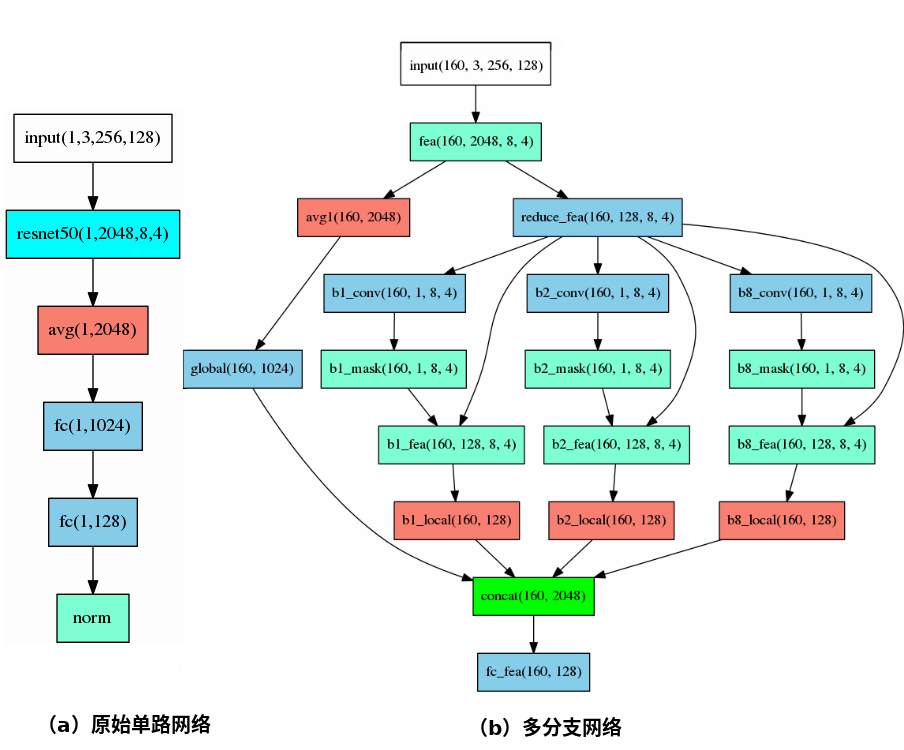
\includegraphics[width=.85\textwidth]{branch.png}
	\caption{空间级别的多分支注意力机制} \label{fig:branch}
\end{figure}

我们使用深度网络提取有鉴别能力的行人特征,
目标是应对各种可能的复杂环境,
包括
相机参数的差异、视角的变化,
行人的非刚性姿态变换,
行人穿着、尺度的变化,
环境的明暗、遮挡等。

面对上述诸多挑战,虽然已经有很多前人的研究成果,比如Guo \etal\cite{guo2018multilevel}和Chang \etal\cite{chang2018factor}通过层次化的方法提取有鉴别能力的行人特征,但是仍然有很多值的考虑地方:

\begin{itemize}
	\item \cite{zhao2017part} 在得到全局的特征之前的同一阶段同时提取局部特征,是否存在信息的冗余?
	      不同的局部特征,比如背包、头发,应该如何与全局特征融合,是使用训练结束就固定的权重,还是使用与输入有关的动态权重?图~\ref{fig:branch}为复现\cite{zhao2017part}的可视化网络结构。
	      % discard?or put to future work?
	\item 对于存在空间失配的再识别问题,采用什么样的注意力机制最为合适?我们观察到\cite{zhao2017part} 每增加一个分支,就会增加许多参数和计算量,如何在引入注意力机制的同时,权衡复杂度与性能之间利弊?
\end{itemize}

在度量学习方面,我们首先在真实数据集上可视化了现有损失函数,分析了各个损失的优缺点。其优缺点总结如下:
\begin{enumerate}
	\item 中心损失对各个类别给以相同的重视程度,但是不同类别之间容易被混淆的程度是不一样的。
	      同时中心损失本身只考虑类内距离,因此单独使用无法做到类间散度最大化;
	\item 
	      如前所述,交叉熵损失基于线性最优分类器的想法,只能在封闭环境下。它学得的决策分界面具有可分性,但不具有鉴别性;
	\item 
	      基于实例的度量损失,如二元组或三元组损失,如果没有在线难样本挖掘的帮助\cite{yaqing2016semantics},仅仅依靠随机选择样本对和更长的训练时间,会导致模型过度强掉简单样本,进而导致性能下降。
	\item 
	      基于实例的度量损失,如三元组损失,如果有难样本挖掘的帮助,就能找到最富有信息的样本,并利用这些代表性的样本实现类间间距最大化,最终获得很好的性能。
	      但是即使考虑了不同类别之间最大化边界,
	      在实验中我们观察到,这种损失泛化到测试集时仍然可能因为某些类别的散度较大,
	      存在一些样本偏离到边界,容易和开放环境下的其他样本或潜在的类中心混淆。
\end{enumerate}

随后我们提出了对比中心损失,联合三元组损失共同监督,端到端地学习了使用深度网络作为核函数的度量函数,
有效提升了行人再识别的CMC-1和mAP指标。

% -------------------------------------------------------------------------
\chapter{基于注意力机制的多尺度特征融合} \label{chap:attention}
% -------------------------------------------------------------------------

\section{问题概述}

\begin{figure}
	\centering
	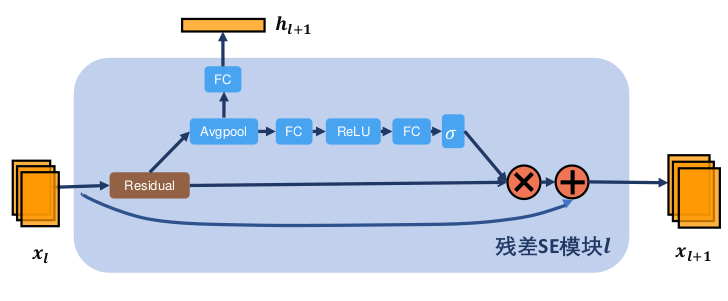
\includegraphics[width=\textwidth]{fig/2018-05-11-16-53-10.png}
	\caption{兼具提取属性特征作用的残差SE模块}
	\label{fig:resse}
\end{figure}

行人再识别旨在学习鲁棒的特征,达到最小化类内间距和最大化类间间距的目标。
但是由于跨摄像头检索时,环境和行人姿态的各种变化,导致模型很难自发地学到具有鉴别能力的特征。
同时,由于检测器的误差,导致行人图片存在一定的空间维度偏移,即空间失配,给行人再识别带来了极大的挑战。
如图~\ref{fig:label2det}所示,我们在CUHK03人工标注数据集和CUHK03检测其自动检测数据集上,训练了相同的基准模型,
在CUHK03人工标注版本的数据集上,基准模型预测结果与期望结果完全一致;而在CUHK03检测器自动检测的数据集上,
由于测试集中的图片存在严重的空间失配,五个预测结果没有一个正确。
其中模型认为最为可能的预测结果,由于受到了询问图片中红色背景的干扰,从候选集中挑选了一张存在红色遮挡物的图片。可见,模型应当将注意力集中于前景区域,从而提取鲁棒的行人特征。对此,我们提出了基于注意力机制的多尺度特征融合方法。其中多尺度机制有助于高分辨率的局部特征在没有信息损失的情况下参与到最终的行人特征表示;注意力机制有助于去除中层属性特征的背景干扰。

传统的工作中通常直接使用深度神经网络的最后一层定义统一的特征空间。
但是想要应对各种变化,中层的局部特征也非常重要\cite{yu2017devil},
于是,我们 
通过注意力机制,抽取、凝练中层属性特征中的重要信息,然后与高层语义特征融合。
我们提出的模型在网络结构上引入先验,从而融合高层语义特征和中层属性特征。
模型包含两个模块:\textbf{(1)、}基于注意力机制的多尺度属性特征提取模块;\textbf{(2)、}特征融合与度量学习模块。

\section{框架设计及算法实现}

\subsection{多尺度属性特征提取模块}

\begin{figure}
	\centering 
	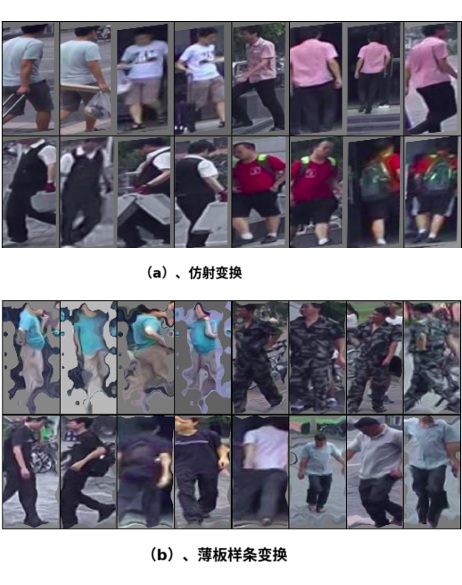
\includegraphics[width=.75\textwidth]{fig/stn1.png}
	\caption{STN的全局变换与局部变换} \label{fig:stn-lc-gl}
\end{figure}

基础的骨架网络采用卷积神经网络结构。可以采用的结构包括残差神经网络(ResNet)\cite{he2016identity}、Inception网络\cite{szegedy2015going}以及Squeeze \& Extraction网络\cite{hu2017senet}等。

为了说明我们方法的有效性,我们采用在ImageNet上预训练好的ResNet-50模型,这是目前最为通用的基础骨架模型。
该模型采用全卷积的架构,即所有的参数层都可用卷积层实现。
一般的方法直接对最后一层卷积层的特征进行全局池化,获得图像的表示$x_4$。
由于在环境、姿态、视角的变化,使用全局特征往往不能很好地鉴别不同的行人,所以
我们同时使用中间层特征来补充$x_4$。
这样的策略,从前向传播的角度看,保证了最终的表示有效包含高分辨率的中层属性信息;从反向传播的角度看,保证了监督信息有效反传更新中层特征,有助于学到更加有鉴别力的表示。

考虑到行人再识别中,姿态的多变、相机视角的差异都会导致严重的空间失配,图像的空间信息不是很可靠,
简单地池化拼接中层属性特征反而会引入背景噪声,造成性能下降,
这一点我们在CUHK03检测数据集上得到了验证。
于是我们引入了在通道层面压缩抽取的注意力机制。
之所以引入通道层面的注意力机制,而不是空间上的注意力机制,是基于以下观察:
\begin{itemize}
	\item 目前主流的分类网络,包括残差网络,都在最后一层采用全局池化,抛弃空间信息。这样的做法导致预训练好的模型倾向于将行人的不同高层语义部件或中层属性特征分布在通道层面,而不是混合在同一通道中。
	\item 可视化深度网络高层的特征图可以发现,它的同一通道的激活值往往具有稀疏性,这种稀疏性不是传统意义上的有很多接近于零的激活值,而是同一个通道内的激活值往往表示同一个概念或者行人部件。因此与其再使用空间层面的注意力,倒不如相信深度网络本身已经实现了在同一通道内集中注意力于一个概念。于是更重要的是对不同的语义部件或属性特征进行有选择性地强调、甚至创造新的语义部件或属性特征来替换不重要的。
	      参考Hu \etal \cite{hu2017senet},我们采用在通道层面压缩和激活的注意力机制。这样的方法在ImageNet分类任务上效果获得了较好的效果。
	      一方面,这种方法能够避免空间信息的噪声干扰,使得最终的特征更为鲁棒;
	      另一方面,这种方法基本不增加计算量和显存开销。	
\end{itemize}

如图~\ref{fig:resse}所示,我们基于\cite{hu2017senet}提出了残差SE模块,用于替换残差网络中的瓶颈模块(Bottleneck Block)。
该模块通过通道级别特征响应的重新组合,自动选择出具有鉴别力的特征或重新组合创造出新的特征,从而将有限的计算资源分配于计算最富有信息量的特征信号分量。
% 公式也许
从计算量的角度看,由于浅层属性特征的通道维度通常较小,增加通道级别的注意力重组机制不需要耗费过多的计算量;
但是高层语义特征的通道维度通常较高,会增加计算量和参数,增加过拟合的风险。
但是幸运的是,通过实验,Hu \etal 发现最终的全局特征
不需要进一步使用通道层面的注意力机制。
因为即使使用了注意力机制
,学习到的注意力权重也接近于均匀分布。
这说明,最终的全局表示在每一个通道上都有特定的语义信息,冗余程度较小,重要程度相同。
遵循这一观察,我们进一步提出在特征融合阶段自适应地重用每个阶段抽取的属性特征$h_{l+1}$。

% \misscite Resource Aware Person Re-identification across Multiple Resolutions
但是我们采用的通道级别的注意力机制不一定是最好的,在之后的实验中也会看到它仍然有缺点,在毕设中我们还尝试了很多其他注意力机制,比如在最后一层特征上使用空间级别的多分支注意力机制(如图~\ref{fig:branch}所示);基于STN变换的注意力机制(如图~\ref{fig:stn-lc-gl}所示)。其中在STN的尝试中,我们发现STN依赖于初始化或者较小的学习率,虽然有一些成功的样例,但是一旦超参数设置的不合理,比较容易训练崩溃。如图~\ref{fig:stn-lc-fail}所示,在失败案例中,已经无法辨识行人。

\begin{figure}
	\centering
	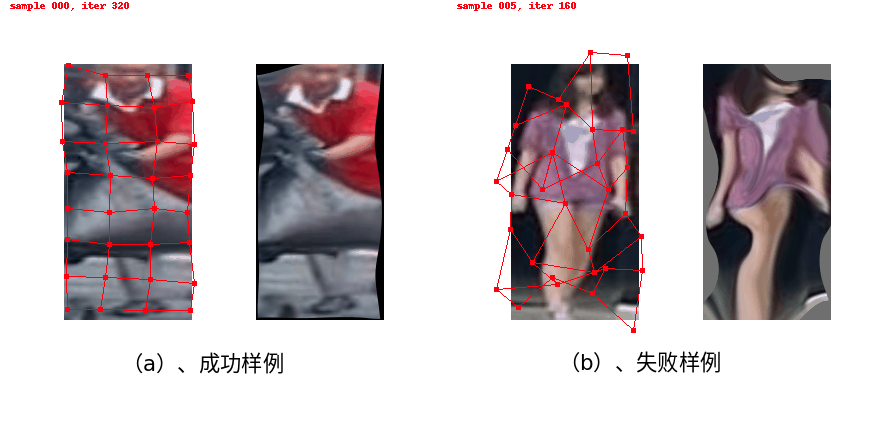
\includegraphics[width=\textwidth]{fig/2018-05-19-23-06-12.png}
	\caption{STN局部变换,即薄板样条变换的可视化样例} \label{fig:stn-lc-fail}
\end{figure}

\subsection{特征融合与度量学习模块}

在特征融合方式上,我们尝试了很多种模式,包括:
\begin{itemize}
	\item 先将中层特征和全局特种嵌入到共享的128维空间,然后自适应求和得到紧凑的特征表示;
	\item 直接将各个层次的特征拼接,引入Dropout机制防止过拟合,通过全连接层的权重自适应地获得128维空间的嵌入表示;
	\item 使用特征本身作为输入求得权重对特征进行变换。这种方法的特性是注意力权重由输入动态决定,但是由于在从特征到权重的过程中不可避免地要学习全连接层权重,这种方式在一定程度上退化为了第二种方法。
\end{itemize}

通过实验,我们最终采用了图~\ref{fig:fusion}的特征融合方式。首先对中层特征进行通道层面的属性特征注意力重组,全局池化抽取中层属性特征,然后与最后的语义表示通过拼接的方式形成最终的特征表示。值得注意的是,在基于注意力机制重新组合特征的过程中,我们已经获得了这一阶段的属性表示。
重用该属性表示,我们既没有引入过多的计算,
又有助于深层监督信息更加容易地反传监督中层属性特征的学习。

\begin{figure}
	\centering
	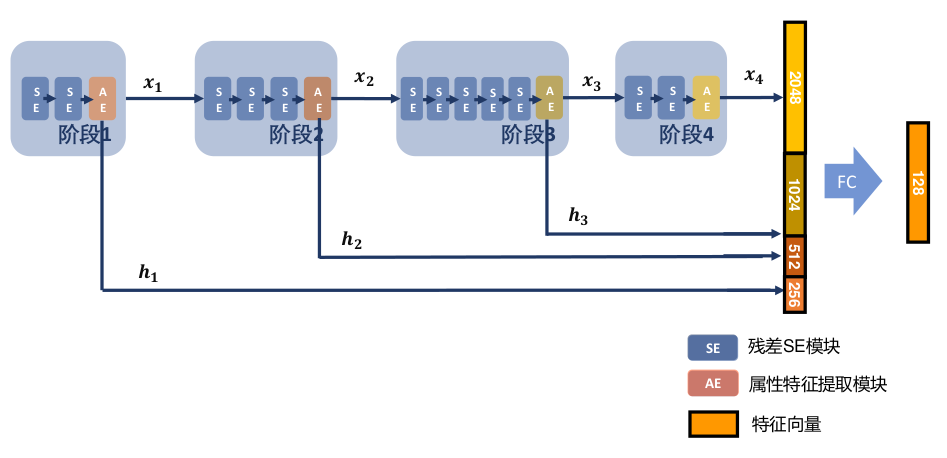
\includegraphics[width=\textwidth]{fig/2018-05-11-16-54-07.png}
	\caption{中层特征与全局特征的融合方式}
	\label{fig:fusion}
\end{figure}

由于我们的目标是直接学习128维度的嵌入特征,因此我们采用了更为合适的度量学习方法---基于难样本挖掘的三元组损失\cite{hermans2017defense}。
在损失计算的过称中,
我们在随机生成的小批次样本集合(mini-batch)中选择最难的样本对$(\mX_a, \mX_p, \mX_n)$,
其中 $(\mX_p, \mX_a)$是属于同一行人的正样本对
, $(\mX_n, \mX_a)$是属于不同行人的负样本对。
我们采用 $\vx_a, \vx_p, \vx_n$表示每个样本经过深度网络获得的
嵌入表示,则基于难样本挖掘的三元组损失如公式~\ref{eq:trihard}所示。

\begin{equation}
	\cL_{\textrm{TriHard}} (\mX, \vtheta) = \sum_{a=1}^{N} \max\left(
	0, m + \min_{\substack{
			p=1...N \\
			y_a = y_p}
	} D(\vx_a, \vx_p)
	-  \max_{ \substack{
			n=1...N \\
			y_a \neq y_n }
	} D(\vx_a,\vx_n)
	\right) \label{eq:trihard}
\end{equation}

其中,难样本体现在求最远的正样本和最近的负样本上。锚点样本会循环遍历整个小批次样本集合,
找到对应的 $\vx_p$嵌入空间中最远最难的正样本和 $\vx_n$ 最近最难的负样本,计算单个样本的损失。
由于该损失存在次梯度较难优化,因此我们通常采用ImageNet预训练好的模型或者是分类任务预训练好的模型初始化,通常使用ImageNet初始化的模型泛化能力较好。
在训练过程中,需要注意观察统计信息$D(\vx_a,\vx_p)$、$D(\vx_a,\vx_n)$随时间的变化。合理的变化应当如图 ~\ref{fig:triok}所示,从特征聚拢在原点开始,
到散布到整个特征空间,过程中$D(\vx_a,\vx_n)$应当普遍比$D(\vx_a,\vx_p)$变换地更快。一旦出现不合理的变化,即特征突然坍塌向原点,就应该立即停止训练。

\begin{figure}
	\centering 
	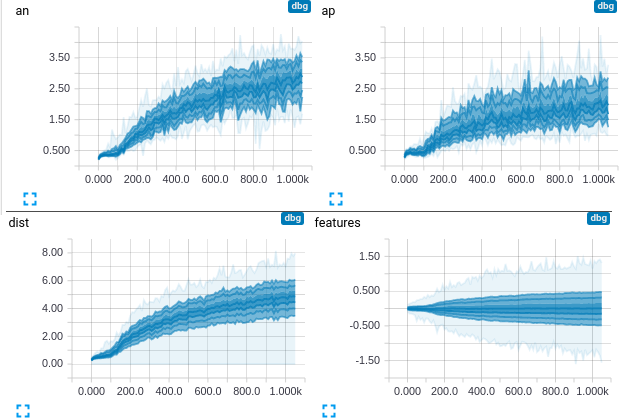
\includegraphics[width=.9\textwidth]{fig/2018-05-19-23-10-33.png}
	\caption{难样本挖掘三元组损失$D(\vx_a,\vx_p)$、$D(\vx_a,\vx_n)$等指标在训练过程中的变化} \label{fig:triok}
\end{figure}

\section{实验设计和结果}

\subsection{数据集信息与评估协议}

我们提出的算法在四个广泛使用的数据集里训练和评测包括CUHK03 \cite{li2014deepreid}, 
Market1501 \cite{zheng2015scalable},  CUHK01 \cite{li2013locally}, 
和DukeMTMC-ReID \cite{zheng2017unlabeled} \cite{ristani2016MTMC} 。
% and VIPeR \cite{gray2007evaluating}。
表~\ref{table:dataset}列出了各个数据集的统计信息和普遍遵循的训练测试划分协议。

\begin{table}
	\centering
	\caption{数据集统计信息和训练测试划分协议}
	\label{table:dataset}
	\begin{tabular}{lllll}
		\toprule
		Dataset    & CUHK03 & Market1501 & CUHK01  & DukeMTMC \\
		\midrule
		identities & 1,467  & 1,501      & 971     & 1,812    \\
		images     & 13,164 & 32,668     & 3,884   & 36,411   \\
		views      & 2      & 6          & 2       & 8        \\
		train IDs  & 1,367  & 751        & 871/485 & 702      \\
		test IDs   & 100    & 751        & 100/486 & 1110     \\
		\bottomrule
	\end{tabular}
\end{table}

\begin{description}
	\item[\textbf{CUHK01数据集}]
	      包含两个摄像头拍摄到的971 个行人,3884 张行人图像,平均每个行人包含来自不同摄像头的图片各两张。两个摄像头之间存在近乎90度的视角变化,因此难度较大。普遍遵循的训练测试划分协议有100 个测试身份和485个测试身份两种版本。为了方便和文献中方法进行比较,我们在两种协议下都做了相应的实验。
	\item[\textbf{CUHK03数据集}]
	      对CUHK01数据集进行了大幅扩充,包含1360个行人,13164张行人图像。它的评估协议有两个版本,
	      分别是人工标注行人边框形成的数据集
	      和DPM行人检测器自动生成边框的数据集
	      。
	      对于检测器自动生成的数据集,平均每个行人拥有10 张图像,平均每个监控视角5张。对于人工标注的数据集,平均每个监控视角每个行人有4.7张图像。
	      同样为了方便比较,
	      我们在两个版本的数据集上都做了实验。
	      % todo cuhk03 new protocol 
	      % \textbf{ViPeR数据集}是一个较小的数据集,
	      % 它包含
	      % 来自两个视角无重叠的623个行人目标。
	      % 每个行人在
	      % 在单个视角里每个行人仅有一张图像。
	      % \item
	      
	      % \textbf{PRID450s数据集}共包含450个行人的900张图片。每个行人都有来自两个室外摄像头的一对图像,摄像头之间的光照、视角、相机参数的差异增加了该数据集的难度。
	      % \item
	      
	      % \textbf{i-LIDS数据集}由在机场到达大厅收集的视频监控构建的,存在一定的行李遮挡情况。它包含119个行人的479张图像,平均每个行人有4张图片。
	      % \item
	      
	      % \textbf{PRID2011数据集}包含从两个固定摄像头里捕捉到行人图像,虽然两个视角各有385和749个行人图像,但是两个摄像头共有的行人只有200个。遵循以往工作,我们采用100个身份作为训练集,剩下个100个作为测试机。
	      % 在测试时,使用一个视角下的100张图像作为查询图像,另一个视角下的100张相同身份的行人图像和剩下所有图像作为搜索库。
	      
	\item[\textbf{DukeMTMC-reID数据集}]是多摄像头追踪数据集DukeMTMC的子集。它也是基于图像的行人再识别数据集,包含1404个至少在两个摄像头中出现过的行人和408个只在一个摄像头中出现的行人。
	      后者用于作为干扰图片。一般使用702个行人训练,702个行人测试。
	      
	\item[\textbf{Market1501数据集}]是一个大规模的行人再识别数据集。由6个几乎参数基本相同的摄像头采集,包含1501个行人,32668个DMP检测器检测的行人图片。该数据集的挑战在于DPM质量比较差,
	      检测框会存在严重的空间失配,同时该数据集相机视角变化较大。通常使用751个行人做训练,750个行人做测试。
\end{description}

为了衡量我们提出的基于多尺度特征融合方法的性能,
我们采用累积匹配因子(Cumulative Matching Characteristics,CMC)指标和mAP指标。
CMC指标衡量了从样本库里找到的样本正确排在查询列表允许预测次数范围内的概率(频次);
mAP指标通过测量不同允许预测次数下的精度的平均,
综合衡量了整个预测列表与预期结果之间的差距。
% todo cmc-1 all protocol mAP


\subsection{实验结果和比较}

% ITML~\cite{itml}, LMNN~\cite{lmnn}, KISSME~\cite{kissme}, LOMO+XQDA~\cite{xqda}, LSSCDL~\cite{lsscdl}, LOMO+LSTM~\cite{lstm}; 
% and DCNN feature based methods: 
% FPNN~\cite{fpnn}, ImprovedDL~\cite{improveddl}, 
% Single-Image and Cross-Images Representation learning (SICIR)~\cite{sicir}, 
% TCP~\cite{tcp}, 
% DCSL~\cite{yaqing2016semantics}, 
% Pose Invariant Embedding (PIE(R)+Kissme)~\cite{pie}, 
% MTDnet (including MTDnet-cross)~\cite{mtd}, 
% JLML~\cite{jlml}. 

\begin{table}
	\centering
	\caption{在数据集CUHK03上的CMC-1,CMC-5,CMC-10性能指标比对}
	% \scalebox{0.95}{
	\begin{tabular}{c|ccc|ccc}
		\hline
		\multirow{2}*{Methods}                     & 
		\multicolumn{3}{c|}{labelled CUHK03}       & 
		\multicolumn{3}{c}{detected CUHK03}                                                                    \\
		\cline{2-7}
		\cline{2-7}
		                                           & r=1     & r=5     & r=10    & r=1     & r=5     & r=10    \\ \hline
		KISSME \cite{kissme}                       & 14.17   & 37.46   & 52.20   & 11.70   & 33.45   & 45.69   \\
		LMNN \cite{lmnn}                           & 7.29    & 19.64   & 30.74   & 6.25    & 17.87   & 26.60   \\
		LOMO+XQDA \cite{xqda}                      & 52.20   & 82.23   & 92.14   & 46.25   & 78.90   & 88.55   \\ \hline
		ImprovedDL \cite{improveddl}               & 54.74   & 86.50   & 93.88   & 44.96   & 76.01   & 81.85   \\
		DCSL (with hnm) \cite{yaqing2016semantics} & 80.20   & 97.73   & 99.17   & -       & -       & -       \\
		JLML \cite{jlml}                           & 83.20   & 98.00   & 99.40   & 80.60   & {96.90} & {98.70} \\ 
		SC-PPMN (with hnm) \cite{mao2018multi}     & {85.50} & {98.20} & {99.50} & {80.63} & 95.62   & 98.07   \\ \hline
		\hline
		TriHard Baseline                           & 84.91   & 98.35   & 99.24   & 81.88   & 96.34   & 98.44   \\
		+ SE Attention                             & 87.28   & 98.50   & 99.18   & 85.50   & 95.90   & 97.69   \\
		+ Multi-Scale Fusion                       & 88.28   & 98.44   & 99.25   & 85.93   & 95.37   & 97.06   \\
		+ Rerank                                   & 96.34   & 99.24   & 99.57   & 91.53   & 98.32   & 98.95   \\
		\hline
	\end{tabular}
	\label{tab:cuhk03}
\end{table}

在CUHK03数据集上,如表~\ref{tab:cuhk03}所示,我们与基于传统手工特征方法的 LMNN~\cite{lmnn},KISSME~\cite{kissme},LOMO+XQDA~\cite{xqda}方法以及
基于深度网络特征方法的 ImprovedDL~\cite{improveddl}, JLML~\cite{jlml}, DCSL~\cite{yaqing2016semantics}, SC-PPMN~\cite{mao2018multi},进行了比较。
历史文献中,CUHK03数据集通常使用cmc-1,cmc-5,cmc-10来进行评估。
在使用SE残差模块替换BottleNeck模块时,我们使用了ImageNet上预训练的模型,因而能够有较大提升。进一步使用多尺度特征融合在手工标注检测框的数据集上也有明显提升;
但是在检测器自动检测的数据集上没有明显提升,这是由空间失配导致的。
考虑到我们通过随机选取询问图片的另一相机视角图片一张来构建测试阶段检索集,
随机选取到的另一相机视角图片一旦存在空间失配,就容易匹配失败。
通过可视化失败案例和对比手工标注数据集和自动检测数据集,我们发现
自动检测数据集中的空间失配会导致
提取到相邻干扰行人的属性特征或者背景的属性特征。
中层属性特征还不具有区分行人的语义部分的能力,同时只通过简单的线性变换(全连接层)就直接用于和全局特征融合,因而很容易混入相邻行人或背景干扰。
于是我们进行了补充实验,对中层属性特征使用更复杂的变换,即使用空间上的注意力机制(增加空间掩模矩阵),确实发现在自动监测的数据集上也获得了明显的提升。

表格中的重排序(Rerank)是一种后处理方法,在近几年逐渐受到重视,提升也越来越明显。
一般的文献中都会同时汇报是否进行重排序的结果,我们也遵循这一规范。
在后续的实验中我们会看到,使用重排序能够大幅度提升mAP指标。
他的作用可以通过图~\ref{fig:rerank}理解,输入ID号为0的行人,红色为原始模型对检索集中每个样本
距离(归一化到$[0,1]$)
,蓝色为重排序之后的距离。
预期的结果应当是图片序号小于8的图片(ID号为0)距离很小,其余图片距离很大。
可以看到重排序通过根据测试阶段检索集中的信息(样本之间的全局相互关系)进一步对预测列表调整,
使得不同图片距离的差异进一步拉大,
从而使得预测列表整体的排序更为合理,大幅度提升mAP指标。
而对于cmc-1指标,重排序的提升较小,这是因为深度网络在训练时的监督信息等价于只使用预测列表中第一个样本,要求第一个样本预测正确,
所以网络在预测列表中的第一个样本时,预测结果相对较准。

\begin{figure}
	\centering 
	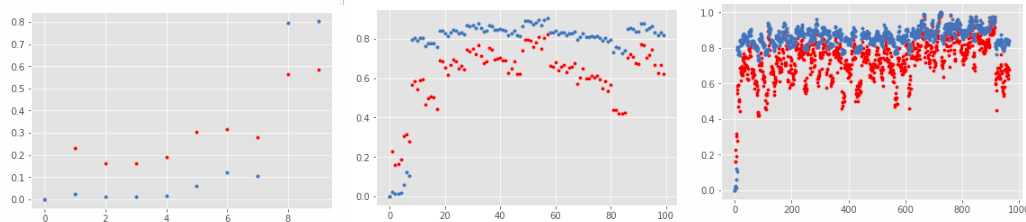
\includegraphics[width=\textwidth]{fig/2018-05-19-23-28-21.png}
	\caption{重排序的作用} \label{fig:rerank}
\end{figure}

\begin{table}
	\centering
	\caption{在数据集Market1501和DukeMTMC上的CMC-1, mAP性能指标对比}
	\label{tab:market}
	\begin{tabular}{c|cc|c|cc}
		\hline
		on Market1501                        & r=1   & mAP   & on DukeMTMC-ReID & r=1   & mAP   \\ \hline 
		SomaNet                              & 73.87 & 47.89 & SVDNet           & 76.70 & 56.80 \\ 
		PAN                                  & 82.81 & 63.35 & PAN              & 71.59 & 51.51 \\  
		TriHard in \cite{hermans2017defense} & 82.99 & 66.63 & TriHard          & 73.24 & 54.60 \\ 
		AWTL                                 & 84.20 & 68.03 & AWTL             & 74.23 & 54.97 \\ \hline  \hline 
		TriHard Baseline                     & 84.62 & 68.68 & TriHard Baseline & 76.32 & 59.57 \\
		+ SE Attention                       & 86.79 & 70.61 & + SE Attention   & 77.29 & 61.12 \\
		+ Multi-Scale Fusion                 & 87.51 & 72.34 & + Multi-Scale Fusion   & 77.12 & 61.64 \\
		+ Rerank                             & 89.19 & 85.08 & + Rerank         & 79.39 & 72.57 \\ \hline
	\end{tabular}
\end{table}


随后我们有在另外两个大型数据集上进行了实验,如表~\ref{tab:market}所示,Market1501和DukeMTMC通常使用cmc-1和mAP指标。
在测量cmc指标时,Market1501的协议会在候选集中加入所有可能的图片,包括干扰图片(垃圾图片)以及空间失配严重的检测结果。
但是Market1501的评估协议中有一项条款使得难度降低了,即只要预测列表中出现了一个正确的答案,后续的答案都算作正确,即不要求把所有匹配图片都预测正确。
因此模型只需要在所有可能的图片中,包括失配不那么严重的图片在内,匹配正确一幅图即可。
这与我们的观察相符,一方面使用Market1501的评估协议得到的cmc-1指标比cuhk03的高;另一方面Market1501上的mAP通常cmc-1低很多,这正是因为mAP考虑的是整体列表
和期望结果之间的差异。
DukeMTMC-ReID上使用和Market1501相同的评估协议。
我们依照\cite{hermans2017defense} 复现了TriHard 基准模型,复现的性能
比原文的中汇报的性能高。
进一步加入注意力机制和多尺度特征融合之后性能也有明显提升,
证明了我们提出方法的有效性。
% todo feature for mrmc ... protocol

\begin{table}[htbp]
	\centering
	\caption{在数据集CUHK01上的CMC-1,CMC-5,CMC-10性能指标比对}
	% \scalebox{0.95}{
	\begin{tabular}{c|ccc|ccc}
		\hline
		\multirow{2}*{Methods}                    & 
		\multicolumn{3}{c|}{CUHK01(100 test IDs)} & 
		\multicolumn{3}{c}{CUHK01(486 test IDs)}                                                              \\
		\cline{2-7}
		                                          & r=1     & r=5     & r=10    & r=1     & r=5     & r=10    \\ \hline
		KISSME \cite{kissme}                      & 29.40   & 60.18   & 74.44   & -       & -       & -       \\
		LMNN \cite{lmnn}                          & 21.17   & 48.51   & 62.98   & 13.45   & 31.33   & 42.25   \\
		LSSCDL \cite{lsscdl}                      & 65.97   & 48.51   & 62.98   & -       & -       & -       \\ \hline
		ImprovedDL \cite{improveddl}              & 65.00   & 89.00   & 94.00   & 47.53   & 71.60   & 80.25   \\
		TCP \cite{tcp}                            & -       & -       & -       & 53.70   & 84.30   & 91.00   \\
		MTDnet-cross \cite{mtd}                   & 78.50   & 96.50   & 97.50   & -       & -       & -       \\
		DCSL (hnm) \cite{yaqing2016semantics}     & 89.60   & 97.80   & 98.90   & 76.54   & 94.24   & 97.49   \\ \hline
		SC-PPMN (hnm) \cite{mao2018multi}         & {93.10} & {98.80} & {99.80} & {77.16} & {92.80} & {97.53} \\ \hline
		\hline 
		TriHard Baseline                          & 88.20   & 98.63   & 99.18   & 73.59   & 85.11   & 89.17   \\
		+ SE Attention                            & 90.43   & 98.23   & 99.55   & 74.92   & 91.37   & 95.82   \\
		+ Multi-Scale Fusion                      & 90.60   & 98.80   & 98.90   & 75.12   & 92.38   & 95.97   \\
		+ Rerank                                  & 96.34   & 99.24   & 99.57   & 79.28   & 95.14   & 97.42   \\ \hline
	\end{tabular}
	\label{tab:cuhk01}
\end{table}


为了验证我们的方法在小型数据集上是否有效,我们在CUHK01上进行了实验。实验发现,我们的方法比基于传统手工特征的方法性能高,
与基于深度网络特征的方法性能相当,
比将手工特征和深度网络特征融合的方法性能稍低。
可见,在小型数据集上手工特征有一定的作用,但是在有足够数据支撑的情况下,
深度网络和注意力机制能获得更好的效果。

% \begin{table}[htbp]
% 	\centering
% 	\caption{在数据集VIPeR和PRID450s上的CMC-1,CMC-5,CMC-10性能指标比对}
% 	%\scalebox{0.95}{
% 	\begin{tabular}{c|ccc|ccc}
% 		\hline
% 		\multirow{2}*{Methods}     & 
% 		\multicolumn{3}{c|}{VIPeR} & 
% 		\multicolumn{3}{c}{PRID450s}                                                                                            \\
% 		\cline{2-7}
% 		                           & r=1            & r=5            & r=10           & r=1            & r=5   & r=10           \\ \hline
% 		KISSME                     & 19.60          & 48.00          & 62.20          & 15.0           & -     & 39.0           \\
% 		LSSCDL                     & 42.66          & -              & 84.27          & 60.49          & -     & 88.58          \\
% 		LOMO+LSTM                  & 42.40          & 68.70          & 79.40          & -              & -     & -              \\
% 		LOMO+XQDA                  & 40.00          & 68.13          & 80.51          & \textbf{61.42} & -     & \textbf{90.84} \\ \hline
% 		\hline
% 		ImprovedDL                 & 34.81          & 63.61          & 75.63          & 34.81          & 63.72 & 76.24          \\
% 		PIE(R)                     & 27.44          & 43.01          & 50.82          & -              & -     & -              \\
% 		SICIR                      & 35.76          & -              & -              & -              & -     & -              \\
% 		TCP                        & 47.80          & 74.70          & 84.80          & -              & -     & -              \\
% 		DCSL                       & 44.62          & 73.42          & 82.59          & -              & -     & -              \\
% 		JLML                       & \textbf{50.20} & 74.20          & 84.30          & -              & -     & -              \\ \hline
% 		SC-PPMN                    & 45.82          & \textbf{74.68} & \textbf{86.08} & 52.08          & 82.58 & 88.36          \\ \hline
% 		TriHard Baseline           &                &                &                &                &       &                \\
% 		+ SE Attention             &                &                &                &                &       &                \\
% 		+ Multi-Scale Fusion       &                &                &                &                &       &                \\
% 		+ Rerank                   &                &                &                &                &       &                \\
% 	\end{tabular}
% 	%}

% 	\label{table:viper}
% 	% \vspace{-1ex}
% \end{table}

% \begin{table}[htbp]
% 	\centering
% 	\caption{在数据集i-LIDS和PRID2011上的CMC-1,CMC-5,CMC-10性能指标比对}
% 	%\scalebox{0.95}{
% 	\begin{tabular}{c|ccc|ccc}
% 		\hline
% 		\multirow{2}*{Methods}      & 
% 		\multicolumn{3}{c|}{i-LIDS} & 
% 		\multicolumn{3}{c}{PRID2011}                                                                                                      \\
% 		\cline{2-7}
% 		                            & r=1            & r=5            & r=10           & r=1            & r=5            & r=10           \\ \hline
% 		ITML                        & 29.00          & 54.00          & 70.50          & 12.00          & -              & 36.00          \\
% 		KISSME                      & -              & -              & -              & 15.00          & -              & 39.00          \\
% 		LMNN                        & 28.00          & 53.80          & 66.10          & 10.00          & -              & 30.00          \\ \hline
% 		\hline
% 		TCP                         & \textbf{60.40} & \textbf{82.70} & 90.70          & 22.00          & 47.00          & 57.00          \\
% 		MTDnet                      & 57.8           & 78.61          & 87.28          & \textbf{32.00} & 51.00          & 62.00          \\
% 		\hline
% 		SC-PPMN                     & 54.80          & 81.92          & \textbf{92.32} & \textbf{32.00} & \textbf{53.00} & \textbf{63.00} \\ \hline
% 		TriHard Baseline            &                &                &                &                &                &                \\
% 		+ SE Attention              &                &                &                &                &                &                \\
% 		+ Multi-Scale Fusion        &                &                &                &                &                &                \\
% 		+ Rerank                    &                &                &                &                &                &                \\
% 	\end{tabular}
% 	%}

% 	\label{table:ilids}
% \end{table}


% \section{本章小结}

% -------------------------------------------------------------------------
\chapter{基于对比中心损失的度量学习}
% -------------------------------------------------------------------------

\section{问题描述}

行人再识别问题是图像检索的子问题,它的输入通常是一些从未在训练集中出现过的行人图片,我们希望最终获得能广泛应用于未知环境、未知行人的距离度量函数。
因此度量学习更适用于行人再识别。

在早期的文献中,度量学习的目标是学习一个相似性函数。通常采用马氏距离
$\norm{\vx_1 - \vx_2}_\mM=
	\sqrt{(\vx_1-\vx_2)^T \mM (\vx_1 - \vx_2) }$
作为相似性度量,学习其中的半正定矩阵$\mM$。
但在最近的文献中,往往使用神经网络自动学习嵌入特征$\vx_1, \vx_2$,同时使用最简单的距离度量---欧式距离。
通过在欧式空间中设计
带有间隔(margin)损失函数
直接学习行人图片在欧式度量嵌入空间中的
特征表示。
因此,从某种程度上来说,现有的度量学习已经转化为了特征学习。
典型的损失函数包括对比损失、三元组损失,
他们都在特征空间中定义了直观的损失函数,使用欧氏距离作为特征空间的度量函数,深度网络作为核函数,端到端地学习图像空间的非线性度量函数。

从是否给每个类别创建模板的角度,损失函数可以分为基于模板的损失和基于实例的损失。
从度量函数的角度,损失函数可以分为基于交叉熵的损失和基于欧式间隔的损失。(虽然交叉熵严格来说不属于度量函数,因为它不具有对称性。但它广泛用于表征两个概率分布之间的距离。)
% 比如Zheng?使用Logistic损失函数对“同一行人的类内距离小于不同行人的类间距离”这一事件的概率建模,得到了PRDC模型。
% 图是怎么来的。。。

我们首先在大型数据集上可视化分析各个损失的优缺点,然后基于实验观察提出对比中心损失。值得一提的是,我们提出的损失函数与现有的最新工作能够相互适应、相互提升,比如进一步引入上一章中注意力机制\ref{chap:attention},或最新的网络结构
\cite{szegedy2015going},\cite{hu2017senet}
, 我们的方法仍能获得进一步的提升。

\section{研究方法}
\subsection{损失函数分类与优缺点分析}

每一种损失都有各自的优缺点,如图~\ref{fig:losses}所示,这是在CUHK03数据集上选取10个类别和对应的全部样本可视化的结果,
红色三角形代表类别中心,
蓝色或黄色圆形代表每一类别的实例。

\begin{figure}
	\centering
	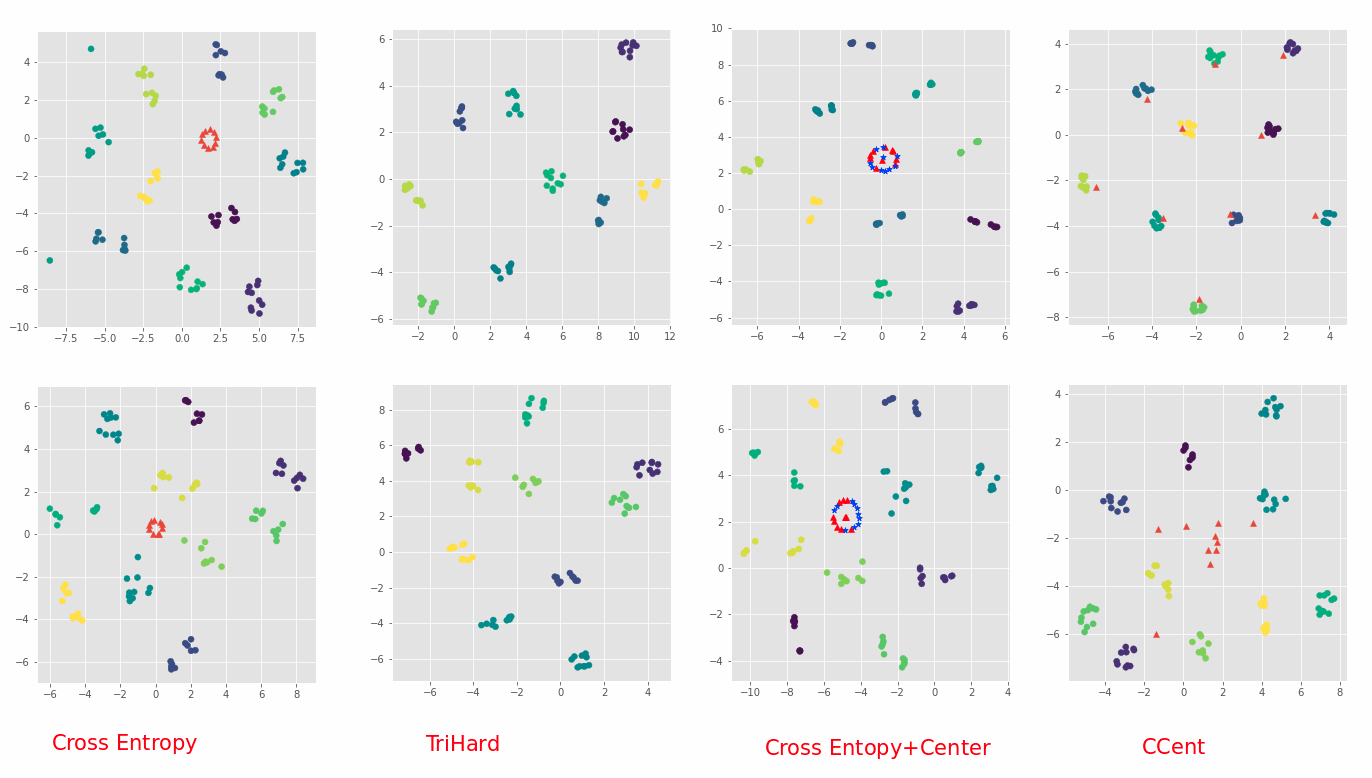
\includegraphics[width=1.1\textwidth]{fig/2018-05-16-15-03-54.png}
	\caption{三种损失函数监督的验证集特征向量和中心向量在2维平面上降维可视化,使用CUHK03数据集和各损失的基准模型得到}
	\label{fig:losses}
\end{figure}

\begin{itemize}
	\item 中心损失虽然成功学到了每个类别的中心,
	      但是对各个类别给以相同的重视程度,而忽略了
	      每个类别区分难易度不同的事实,
	      因此部分类心很容易与临近的类心混淆;
	      除去每个类别区分难易度不同,还存在一些标注错误或实在困难的样本容易和临近类心混淆。
	      对于这类样本,与其使用相同的权重使得它尽可能接近类心,倒不如忽视这类样本防止过拟合,以便获得一个对大部分样本泛化能力好的特征提取器。
	\item 传统的基于模板的损失具有较高的计算效率,因为它会为每个类别创建学习模板,而这样的模板包含了整个数据集中某一类别的所有信息,且随着深度网络的训练不断被迭代更新。
	      它在ImageNet大规模分类时代做出了重大贡献。但是对于再识别问题,它有一定的缺点。
	      如图~\ref{fig:losses}所示,将交叉损失的分类器权重视作类心向量与样本特征向量共同嵌入到2维空间可视化,
	      我们看到在训练集上
	      存在一些蓝色样本点,仅仅只是被分在了类心定义的分界超平面内部,而没有聚拢成一类。
	      这样损失监督训练的模型提取的特征向量会很容易
	      与相邻类别混淆。
	      这就是所说的具有可分性,但是不具有鉴别性。
	      这样的特征向量只能用于封闭环境的分类问题,无法适应开放环境的再识别问题。中心损失与交叉熵损失的对比可以进一步在图~\ref{fig:distmat-all}中看到,从右侧上方的样本中心的距离矩阵看,中心损失使得一个样本能够找到对应最近的中心,容易混淆的中心也只有几个;而交叉熵损失的模板权重,只是确定不同类别的方向,因此不会真正成为类别的中心。
	\item 三元组损失关注样本对之间的细粒度的关系,样本级别的关系有时候会比样本与模板之间的关系包含更多信息。
	      基于难样本挖掘的三元损失成功挖掘了这样的信息,
	      为不同的类别拉开了一定的距离,但是仍然具有较大的类内散度。
	      尤其对于再识别问题,明显地看到它倾向于将同一行人的两个摄像机视角的图片聚成两个类别。 
	      基于难样本挖掘的三元组损失的缺点可以进一步在图~\ref{fig:tsne}中观察到,尽管验证集上的类内散度已经很小了,
	      但是由于在测试集上存在一些样本偏离到边界,
	      容易和临近的类别混淆。
	      就是这样的一些样本造成了性能指标的下降。
\end{itemize}

\begin{figure}
	\centering 
	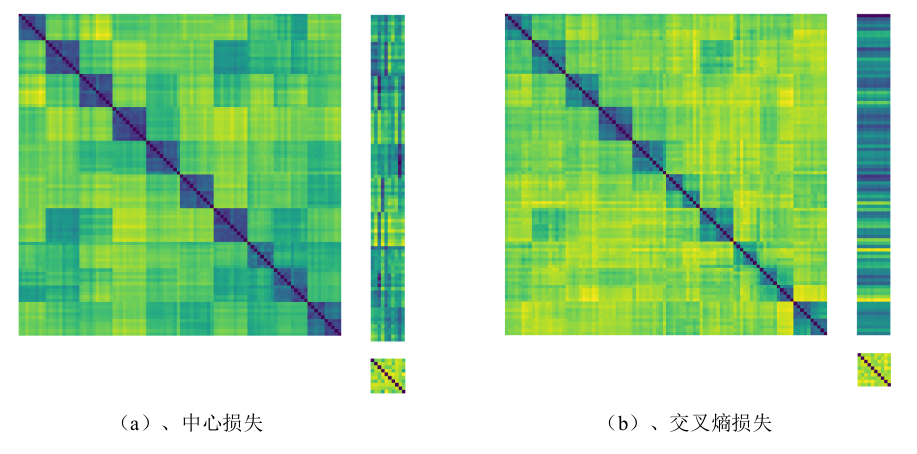
\includegraphics[width=\textwidth]{fig/2018-05-20-14-43-35.png}
	\caption{不同损失的类别样本距离矩阵、样本中心距离矩阵以及中心混淆矩阵} \label{fig:distmat-all}
\end{figure}

\begin{figure}
	\centering
	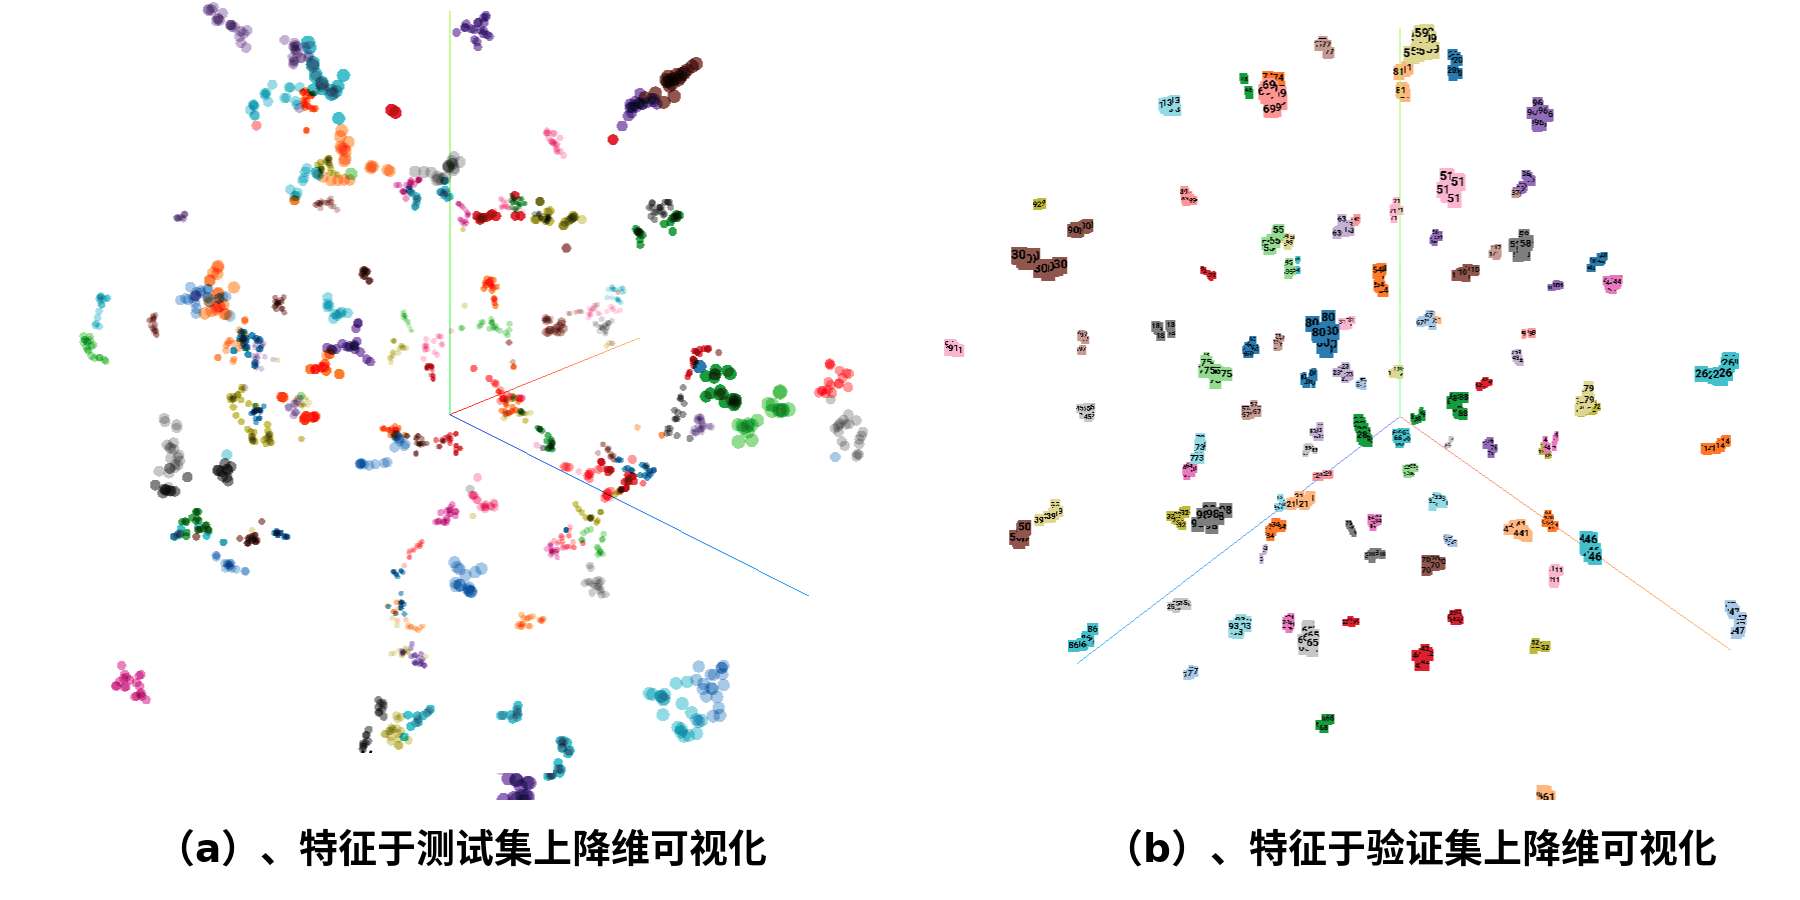
\includegraphics[width=\textwidth]{fig/tsne.png}
	\caption{三元组损失在3维空间降维可视化,使用CUHK03数据集和我们的基准模型得到}
	\label{fig:tsne}
\end{figure}


\subsection{对比中心损失}

首先对我们所采用的符号进行说明。
假设训练集可以表示为$\cT=\{(\mX_i,y_i)\}_{i=1}^{N^{\textrm{train}}}$, 由$N^{\textrm{train}}$个图片样本
$\mX_i \in \real^{W\times H\times C}$
% with $\vx_i \in \real^{F}$ 
和M个类别的
标签$y_i \in \{1,\dots, M\}$组成。
最近一些文献中度量学习的目标可以总结为
学习一个特征提取函数
$\vx = \vf_\vtheta (\mX): \real^{W \times H\times C} \rightarrow \Rbb^D$,
将语义上相似的点从原始数据流形映射到
特定度量(通常是欧氏度量)下相近的点。
一般形式的特定度量可以表示为$D( \vx_i, \vx_j):\Rbb^D \times \Rbb^D \rightarrow \Rbb$,
通常采用的欧式度量为
$D(\vx_i,\vx_j)=\|\vx_i - \vx_j\|_2^2$。
如果特征空间中的度量函数采用
$D(\vx_i,  \vx_j)$的形式,那么在图像空间中的度量函数可以表示为
$D(\vf_\vtheta(\mX_i), \vf_\vtheta(\mX_j))$。
在后续的叙述中,为了简化公式我们会采用$D(\vx_i,  \vx_j)$的表达形式,
看起来它是没有需要训练的参数,
但是事实上$\vx$ 是被 $\vtheta$参数化的,也即损失会通过欧式度量反向传播更新特征提取网络的参数。
类似地,
为了简化公式,我们会采用
$D(\vx_i,\vc_j)$表示样本和中心在特征空间的距离
,而不是$D(\vf_\vtheta(\mX_i), \vc_j)$。

\begin{figure}
	\centering 
	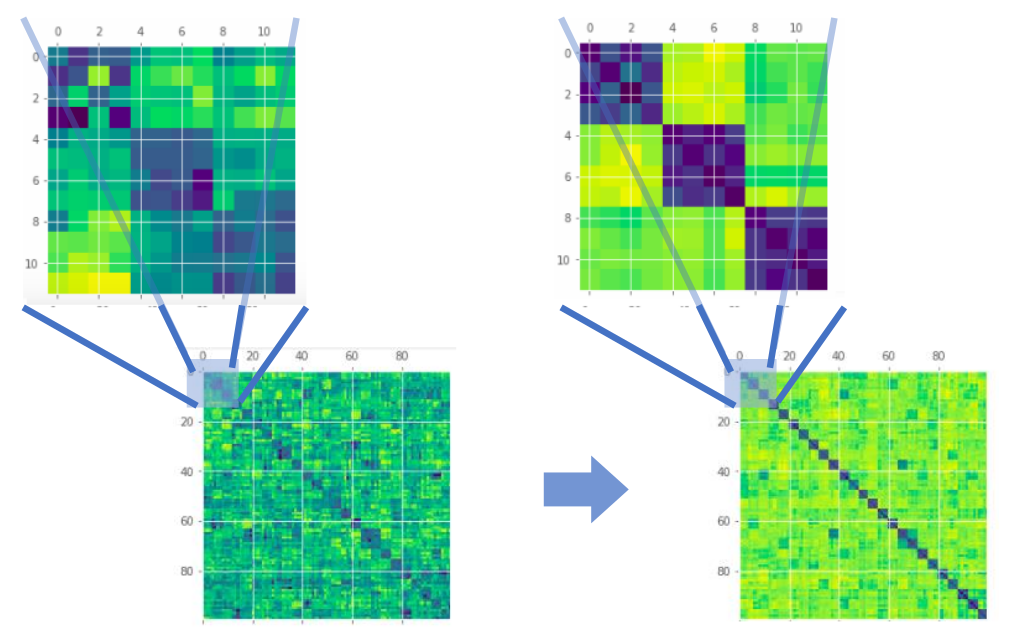
\includegraphics[width=\textwidth]{fig/2018-05-19-23-27-39.png}
	\caption{从距离矩阵学习的角度理解难样本挖掘三元组损失} \label{fig:distmat-tri}
\end{figure}

与第\ref{chap:attention}章相同,我们仍然采用基于难样本挖掘的三元组损失作为基准模型。其公式参见\ref{eq:trihard} 。这里从另外一个角度来理解该损失函数。 如图~\ref{fig:distmat-tri}所示,该损失
的总体目标是将原本混乱距离矩阵转化为特征空间中按类别聚类的距离矩阵。
但是学习整个矩阵,一方面计算量巨大,另一方面模型很容易被一些容易的样本对迷惑,造成梯度信息的消失,这一点在
正负样本对不均衡的再识别问题中尤为严重。因此三元损失需要引入难样本挖掘来辅助学到更好特征。
在实践中,我们观察到
在训练后期,这类基于实例的损失还是不可避免地会饱和,并且出现大量零梯度。这是因为尽管使用了批样本内部的挖掘,但是形成批样本的过程仍然是随机的。于是,有可能出现的情况是:在训练后期,形成的一整个批样本都不包含有效三元组,即所有三元组都已经满足公式
\ref{eq:trihard}
所定义的间隔要求。
而这个现象在CUHK03数据集上尤为突出,因为这个行人再识别数据集包含很多不同的行人,同时每个行人的训练正样本只有不到10张(平均9.4张)。
基于这个观察,我们将结合基于模板的损失,在形成批样本的时候引入难类别挖掘,消除基于实例的损失训练饱和的问题。

我们首先尝试中心损失,这种损失直接使用欧式度量来学习每个类别的中心$\vc_{y_i}$,并将对应类别的样本$\vx_i$拉向中心$\vc_{y_i}$。
\begin{equation}
	\cL_{\textrm{Cent}} (\mX, \mC, \vtheta) = \frac{1}{2}
	\sum_{i=1}^{N}  D(
	\vx_i , \vc_{y_i} )
\end{equation}

\begin{figure}
	\centering
	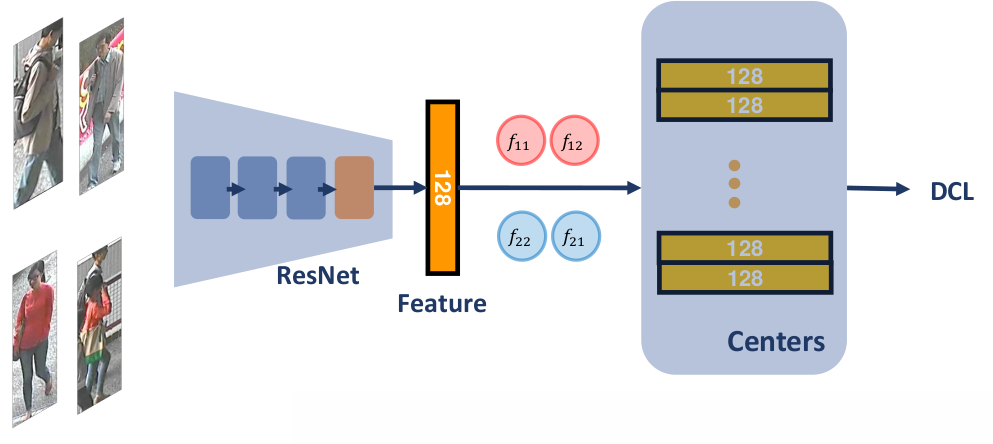
\includegraphics[width=\textwidth]{fig/2018-05-19-22-25-00.png}
	\caption{
		基于对比中心损失的行人再识别总体框图
	}
	\label{fig:dcent}
\end{figure}

\begin{figure}
	\centering
	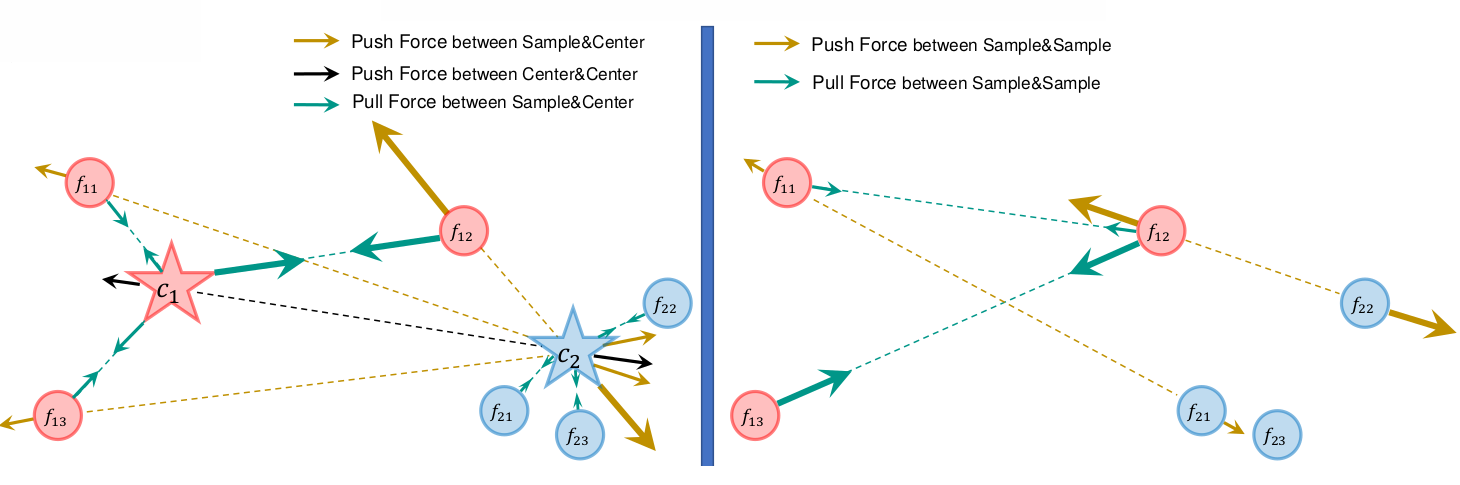
\includegraphics[width=1.1\textwidth]{fig/2018-05-19-22-25-11.png}
	\caption{
		\textbf{左图:}对比中心损失示意图;\textbf{右图:}难样本三元损失函数示意图
	}
	\label{fig:dcent2}
\end{figure}

但是这种损失仍然面临着正样本不足,没有足够的统计信息更新中心模板的问题。
同时这种损失隐式地给每个样本-中心对赋予了相同的权重,显然不符合真实世界的数据分布。
于是我们提出了对比中心损失,其示意图参见图~\ref{fig:dcent}、图~\ref{fig:dcent2},表达式参加式子~\ref{eq:ccent}。

\begin{equation}
	\cL_{\textrm{CCent}} (\mX, \mC, \vtheta) = \frac{1}{2}
	\sum_{i=1}^{N}
	\frac{D(
		\vx_{i}, \vc_{y_i}
		)}{ 
		\displaystyle \lambda_s
		\min_{\substack{
				j=1...M \\
				j \neq y_i }}
		D(
		\vx_{i}, \vc_{j}
		) + 1 }
	-
	\lambda_d \sum_{i=1}^{M}  \min_{j=1...M} D(\vc_i,\vc_j)
	\label{eq:ccent}
\end{equation}

式子~\ref{eq:ccent}中涉及到两个超参数$\lambda_s$和$\lambda_d$;两种类型的推力和一种类型的拉力。

$\lambda_s$用于对样本和正类中心之间的距离进行缩放。
当$\lambda_s$趋近于0时候,中心对比损失退化为中心损失;
当$w_s$趋近于1时,中心对比损失表现地和交叉熵损失较为类似。
$\lambda_d$用于对类心间推力的进行缩放。

$\min_{\substack{
			j=1...M \\
			j \neq y_i }} D(
	\vx_{i}, \vc_{j}
	)$
为样本到最近的负类中心的距离。
$D(
	\vx_{i}, \vc_{y_i}
	)$
为样本到正类心的距离。两者可以看作相互加权,相互动态调整重要性。对比的思想就体现在这里。
如图~\ref{fig:dcent}所示,图中线的粗细表示力的大小。
图中样本$\vf_{12}$和负类中心$\vc_2$很接近,因此样本$\vf_{12}$容易混淆到负类$\vc_2$。
这时,如果将拉力看作推力的权重系数,那么推力会被放大;如果将推力看作拉力的权重系数,则拉力会被放大。对比中心损失根据数据分布本身的特性,动态地给不同的距离以不同的权重。
在前向传播时候,它会多考虑一个负类中心,有助于将损失归一化到一定的范围内。
从反向传播的角度看,多考虑一个负类能提高样本的利用效率。
因为使用一个样本同时更新了正类和最难的负类,加快了类别中心的学习进程。
考虑到大多数的再识别任务中,类别数目可以达到1k,甚至4k。我们只选取最难的负类来减少反向传播时候的计算量。
在实验中我们也观察到,一个样本只会被误判为少数几个身份,因此选取最难的负类中心,已经提供了绝大部分信息,不会使性能下降。

对于类心之间的推力,为了避免相同的类心对不断地被优化(这样的类别中心往往是由标注错误产生的异常类别),
我们对所有类心对中距离最小的$\min_{j=1...M} D(\vc_i,\vc_j)$进行优化。
这是所有可能的类心对中最容易被混淆的一对。
由于随机选取批梯度(每次会有不同类别的样本进入批样本),
加上每次只取最容易被混淆的一对优化,
我们可以有效避免深度网络过度强调特定的类心对。
这一项可以看作对类心权重模板的正则化,
使得类心模板尽可能均匀地散布在特征空间。


\section{结果验证和分析}

\begin{table}
	\centering
	\caption{在数据集CUHK03上的CMC-1,CMC-5,CMC-10性能指标比对}
	% \scalebox{0.95}{
	\begin{tabular}{c|ccc|ccc}
		\hline
		\multirow{2}*{Methods}                     & 
		\multicolumn{3}{c|}{labelled CUHK03}       & 
		\multicolumn{3}{c}{detected CUHK03}                                                                    \\
		\cline{2-7}
		\cline{2-7}
		                                           & r=1     & r=5     & r=10    & r=1     & r=5     & r=10    \\ \hline
		KISSME \cite{kissme}                       & 14.17   & 37.46   & 52.20   & 11.70   & 33.45   & 45.69   \\
		LMNN \cite{lmnn}                           & 7.29    & 19.64   & 30.74   & 6.25    & 17.87   & 26.60   \\
		LOMO+XQDA \cite{xqda}                      & 52.20   & 82.23   & 92.14   & 46.25   & 78.90   & 88.55   \\ \hline
		ImprovedDL \cite{improveddl}               & 54.74   & 86.50   & 93.88   & 44.96   & 76.01   & 81.85   \\
		DCSL (with hnm) \cite{yaqing2016semantics} & 80.20   & 97.73   & 99.17   & -       & -       & -       \\
		JLML \cite{jlml}                           & 83.20   & 98.00   & 99.40   & 80.60   & {96.90} & {98.70} \\ 
		SC-PPMN (with hnm) \cite{mao2018multi}     & {85.50} & {98.20} & {99.50} & {80.63} & 95.62   & 98.07   \\ \hline
		\hline
		Xent                                       & 76.93   & 95.16   & 97.76   & 71.67   & 91.36   & 95.34   \\
		+LblSmth                                   & 78.64   & 93.96   & 96.78   & 75.87   & 91.53   & 95.15   \\ 
		+Cent                                      & 82.21   & 95.55   & 98.39   & 80.12   & 95.38   & 98.11   \\  	
		% CCent                                      & 17.51   & 43.11   & 59.72   &         &         &         \\ 	 
		TriHard                                    & 84.50   & 98.49   & 99.24   & 82.48   & 97.15   & 98.38   \\
		+CCent                                     & 87.77   & 98.70   & 99.55   & 84.86   & 97.61   & 98.48   \\
		+CCent+Dis                                 & 88.12   & 98.80   & 99.40   & 84.45   & 97.15   & 98.44   \\   \hline 
		\hline
	\end{tabular}
	\label{tab:cuhk032}
\end{table}

我们首先在传统的CUHK03上进行实验,如表~\ref{tab:cuhk032}所示,
交叉熵在检索任务上性能较差,即使使用了标签平滑的正则化方法,
性能也仍然无法超过难样本挖掘的三元组损失。
由于交叉熵损失的交叉熵度量函数与中心损失的欧式度量不匹配,
联合监督训练之后性能提升不明显。
当中心损失的权重为0.01时,性能提升,其结果填写在表格中;
当中心损失的权重为0.1时,性能比只用交叉熵还要低。这说明中心损失对超参数比较敏感。另一方面,通过可视化,我们发现性能提升时,学习到的反而不是中心,进一步说明了中心损失与交叉熵损失的不匹配。 
% todo 单独使用我们提出的对比中心损失,
当我们提出的对比中心损失和三元损失联合监督时,获得了很大的提升,同时通过可视化,如图\ref{fig:losses}所示,训练集上的中心为
欧式意义上的$L_2$中心,无论是测试集还是训练集,提取的特征都聚成了一类。尤其是对于再识别问题,两个摄像机视角由于差异较大,往往容易被聚成两个类别,而我们的方法很好地将同一行人的不同摄像机视角图片在特征空间中聚成了一类,真正学到了对视角变化鲁棒的行人特征。

\begin{table}
	\centering
	\caption{在数据集Market1501和DukeMTMC上的CMC-1, mAP性能指标对比}
	\label{tab:market2}
	\begin{tabular}{c|cc||c|cc}
		\hline
		on Market1501                          & r=1   & mAP   & on DukeMTMC-ReID & r=1   & mAP   \\ \hline 
		SomaNet \cite{zheng2017ped}            & 73.87 & 47.89 & SVDNet           & 76.70 & 56.80 \\ 
		PAN \cite{barbosa2017looking}          & 82.81 & 63.35 & PAN              & 71.59 & 51.51 \\  
		TriHard in \cite{hermans2017defense}   & 82.99 & 66.63 & TriHard          & 73.24 & 54.60 \\ 
		AWTL        \cite{ristani2018features} & 84.20 & 68.03 & AWTL             & 74.23 & 54.97 \\ \hline  \hline 
		Xent                                   & 84.92 & 65.15 & Xent             & 72.44 & 51.16 \\ 
		+LblSmth                               & 89.46 & 72.18 & +LblSmth         & 79.08 & 59.80 \\ 
		+Cent                                  & 82.42 & 61.77 & +Cent            & 73.81 & 53.29 \\ 
		TriHard                                & 86.55 & 69.98 & TriHard          & 75.08 & 57.10 \\
		+CCent                                 & 89.12 & 71.57 & +CCent           & 81.54 & 62.33 \\
		+CCent+Dis                             & 90.37 & 72.94 & +CCent+Dis       & 80.36 & 60.87 \\  \hline 
	\end{tabular}
\end{table}

在另外两个大型数据集上,也获得了明显的提升。
如表~\ref{tab:market2}所示,由于Market1501数据集比较特殊,每个行人具有充足的训练数据,因此使用交叉熵损失,辅之以标签正则化,获得了很高的性能。使用我们提出的对比中心损失也获得了具有竞争力的效果。
% todo feature for mrmc ... protocol
% todo AWTL

\begin{table}
	\centering
	\caption{在数据集 iLIDS-VID和Mars上的CMC-1, mAP性能指标对比}
	\label{tab:mars2}
	\begin{tabular}{c|cc||c|cc}
		\hline
		on  iLIDS-VID              & r=1   & r=5   & on Mars    & r=1   & mAP   \\ \hline  
		%    &       &       & TriHard in \cite{hermans2017defense} & 79.8  & 67.7  \\ 
		See  \cite{zhou2017see}    & 55.2  & 86.5  & See        & 70.6  & 50.7  \\  
		ASTPN \cite{xu2017jointly} & 62    & 86    & ASTPN      & 44    & -     \\ 
		Xent                       & 52.28 & 85.71 & Xent       & 74.51 & 74.53 \\
		% +Cent                      &       &       & +Cent                                &       &       \\ 		
		TriHard                    & 66.01 & 91.33 & TriHard    & 80.87 & 74.03 \\
		% +CCent                     & & & +CCent                               & & \\
		+CCent+Dis                 & 68.57 & 92.14 & +CCent+Dis & 82.79 & 77.24 \\  \hline 
	\end{tabular}
\end{table}

在对比中心损失的实验中,我们还在基于视频片段的再识别任务数据集上进行了测评。由于视频数据集数据量较大
,所以我们简单采用了之前实验得到的最好的超参数,
轻松获得了明显提升,证明了对比中心损失的有效性。

% -------------------------------------------------------------------------
\chapter{结论与展望}
% -------------------------------------------------------------------------

\section{结论}

在本次毕设中,我们提出了基于注意力机制的多尺度特征融合和基于对比中心损失的度量学习方法。
前者的动机为:通过可视化失败案例,我们发现在失配严重的数据集上,简单地使用全局特征和局部属性特征拼接,有时候反而会造成性能下降。
于是我们提出了对局部特征进行属性提取来应对失配问题的方法,通过合理地使用注意力机制,我们在计算量没有大幅增加的情况下,获得了性能的提升。
后者的动机为:基于难样本挖掘的三元损失虽然取得了较好的效果,但是可视化发现,该损失只关注局部特性,导致同一行人的两个摄像机视角常常聚成两个类别。
于是我们提出了对比中心损失,灵活地进一步缩小类内间距。
我们在不同大小、难度和类型的数据集上对提出的两种方法进行了实验,性能普遍获得了提升。

\section{毕设中遇到的问题与思考}

在实现再识别算法的过程中,深刻感受到了Python的缺点。比如对每个询问图片计算cmc得到最终cmc指标的过程,不能向量化,只能用for循环实现。导致它在大型数据集上速度很慢。
因此无论将来是做学术还是工程,学习Python和C混编都有一定的意义。

在实验中,我们曾经遇到三元损失训练坍塌到平凡解或者即使收敛性能也很低的问题。
后来通过增加批归一化(BatchNormalize),交叉熵预训练,自步学习等技巧解决。
如图~\ref{fig:trival}所示,在没有使用上述技巧时,训练坍塌;在使用之后,可以复现原文的性能。
不过有意思的是,在人脸识别中,
$L_2$-Softmax提出使用$L_2$归一化的特征向量有助于稳定深度网络和提升性能。
但是在实验中,我们发现稳定深度网络的关键因素是对维度变换前的2048维向量进行批归一化(BatchNormalize),
至于是否对最终的128维特征向量使用$L_2$归一化,
无论是对是否收敛、还是收敛后的性能,都没有绝对的影响。

\begin{figure}
	\centering
	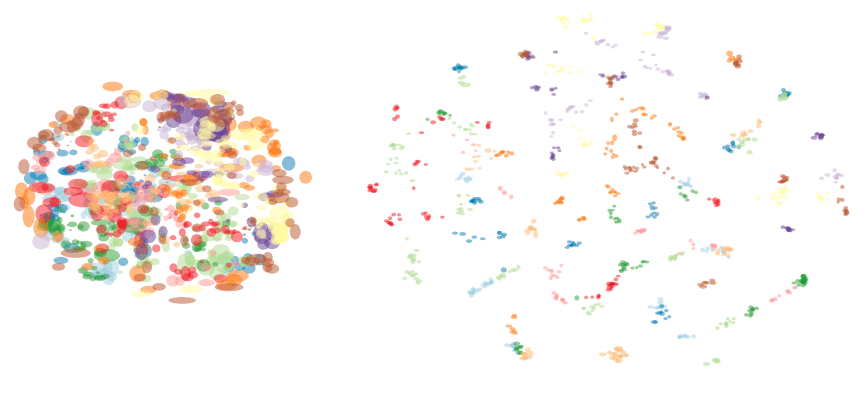
\includegraphics[width=\textwidth]{fig/2018-05-21-10-49-27.png}
		\caption{\textbf{左图}:训练失败;\textbf{右图}:成功收敛}
		\label{fig:trival}
\end{figure}

在实验中,我们尝试了对卷积模块进行设计。
首先我们对卷积的平移不变性进行了理解。
深度学习中的卷积操作是数学意义上的相关性操作,
同时在平移图像时,我们通常丢弃超出边界的像素值,而不是补零扩大图像。
因此,如图~\ref{fig:gconv}所示,对原始图片平移得到的特征图确实具有平移相似性,因为边缘效应可以忽略。
但是如果平移卷积核,所得到的特征图将不具有平移相似性。
随后我们探索了通过参数共享实现卷积的旋转不变性,但是由于群论的知识不足,还是先暂时回到行人再识别的主要课题上探索了。希望之后多补充一下数学知识。

\begin{figure}
	\centering
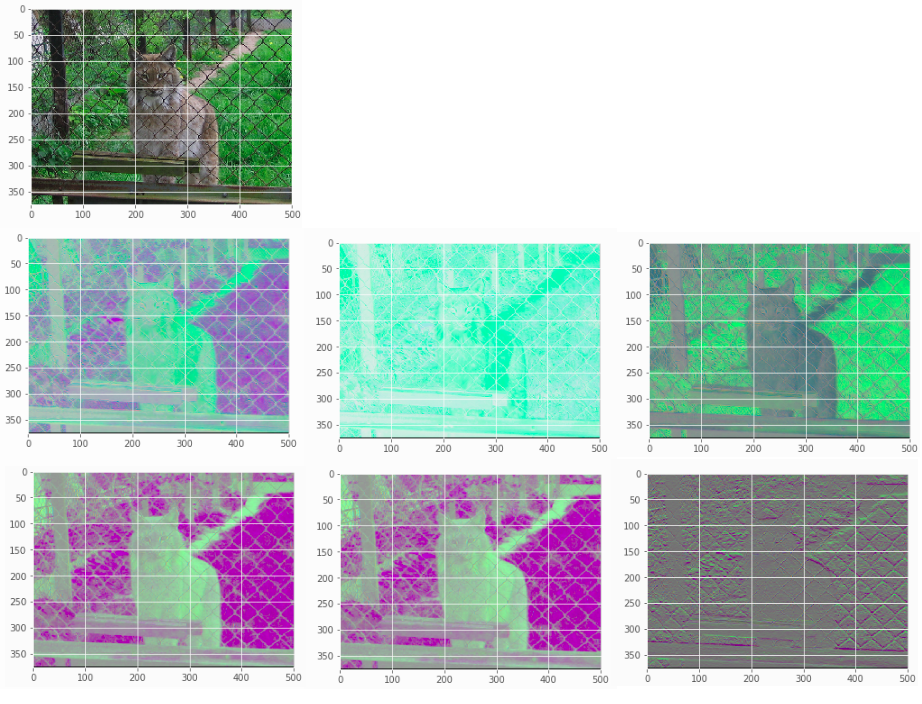
\includegraphics[width=\textwidth]{fig/2018-05-21-10-51-51.png}	
		\caption{平移卷积核是否与平移图像等价。\textbf{第一行}:原图;
		\textbf{第二行}:平移卷积核所得特征图及其差;\textbf{第三行}:平移原图所得特征图及其差。}
		\label{fig:gconv}
\end{figure}

\section{展望}

我们还尝试了使用STN对失配进行校正的方法,发现STN存在一定的缺陷。
如果和其他任务一起训练,它需要一个良好的初始化和较小的学习率,才能稳定收敛;
它也可以通过分阶段训练来稳定,即先将特征提取网络预训练至收敛,然后插入STN进一步调优。类似地,现在很多高层的任务,
都是将提取特征作为一个独立的训练阶段,然后使用预训练的特征提取器实现后续富有想象力的任务。于是,我们的思考是:究竟有没有必要进行端到端的训练、
阻碍行人检测与行人再识别或者其他任务共同训练的难点在哪里、预处理和后处理是否也是很重要?

面对海量视频数据集,我们有没有可能在小型数据集上训练出一个评估网络,用于快速评估给定样本的上下文时的样本信息量,
从而当泛化到海量视频数据集上时,能快速选择有价值的样本进行训练?%也许这和元学习会有一定的联系。

% 如何关注样本间的信息?

深度网络被认为是一个黑盒子,基于交叉熵的分类模型已经有许多可视化方法,图~\ref{fig:grad}基于梯度信息寻找行人图片中对预测结果影响最大的部件(显著性图),可以看到,无论尺度姿态如何变化,衣服的特征都是鉴别该行人的明显特征。基于度量学习的可视化方法仍然较少。也许我们可以从可视化中中得到一些启发 。

% 后续我们继续尝试从虚拟对抗样本提升鲁棒性的角度解释角度损失、动态间隔的三元组损失。
% 这两种损失可以看作在特征空间加入了局部平滑性先验。
% 一些可视化结果如图所示。
% 图~\ref{fig:grad}为基于梯度信息寻找行人图片中对预测结果影响最大的部件,无论尺度、姿态,衣服的特征都是鉴别该行人的明显特征。
% 图~\ref{fig:adv}为加入对抗噪声使得图片匹配失效。深度网络能够通过对输入图片加随机扰动获得一定的
% 鲁棒性,但是真正具有挑战性的噪声应当是加在行人的具有鉴别力的部件上的。从而使得这些部件在大尺度变化之后,深度网络仍然能匹配正确。我们计划通过损失函数的设计达到这一效果。

\begin{figure}
	\centering
	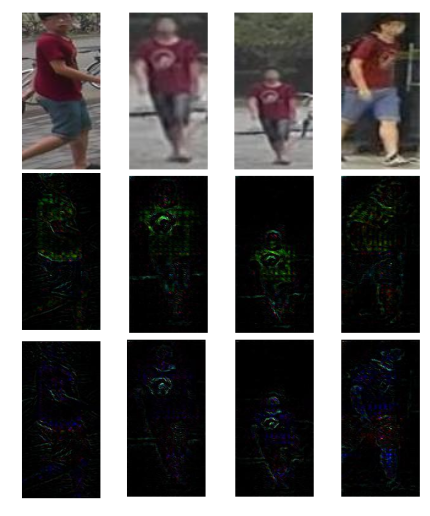
\includegraphics[width=.7\textwidth]{fig/2018-05-21-09-58-23.png}
	\caption{基于梯度的显著性可视化}\label{fig:grad}
\end{figure}

% \begin{figure}
% 	\centering
% 	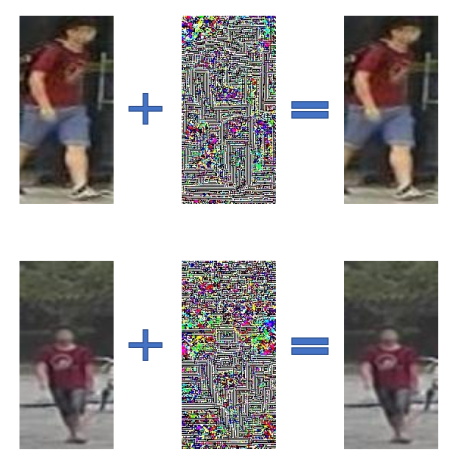
\includegraphics[width=.8\textwidth]{fig/2018-05-21-10-31-13.png}
% 	\caption{从对抗样本看深度网络的可解释性和鲁棒性}\label{fig:adv}
% \end{figure}

\printbibliography[heading=chapbib]
